%%%%%%%%%%%%%%%%%%%%%%%%%%%%%%%%%%%%%%%%%%%%%%%%%%%%%%%%%%%%%%%%%%%%%%%%%
%                                                                       %
% ustthesis_test.tex: A template file for usage with ustthesis.cls      %
%                                                                       %
%%%%%%%%%%%%%%%%%%%%%%%%%%%%%%%%%%%%%%%%%%%%%%%%%%%%%%%%%%%%%%%%%%%%%%%%%

\documentclass{ustpqe}

\usepackage{latexsym}
    % Use the "latexsym" package when encountering the following error:
    %   ! LaTeX Error: Command \??? not provided in base LaTeX2e.
\usepackage{epsf}
    % Use the "epsf" package for including EPS files.

\usepackage{algorithm}
\usepackage{algorithmic}
\usepackage{amsmath}
\usepackage{amssymb}
\usepackage{booktabs}
\usepackage{caption}
\usepackage{graphicx}

\usepackage{subfigure}
%\usepackage{hyperref}
\usepackage{multirow}
\usepackage{rotating}
\usepackage{theapa}
%\usepackage{natbib}
\usepackage{epsfig}
\usepackage[a4paper,top=2.5cm,bottom=2.5cm,left=2.5cm,right=2.5cm]{geometry}
\usepackage{url}
\usepackage[usenames, dvipsnames]{color}


\numberwithin{algorithm}{chapter}
%\renewcommand{\theHalgorithm}{\arabic{chapter}.\arabic{algorithm}}

\def \cite{\shortcite}
\def \citep{\shortcite}


%\def \cite{\cite}
%\def \citep{\cite}


%\input{TexFile/defs}
%%%%%%%%%%%%%%%%%%%%%%%%%%%%%%%%%%%%%%%%%%%%%%%%%%%%%%%%%%%%%%%%%%%%%%%%%
%                                                                       %
% Preambles. DO NOT ERASE THEM. Change to suite your particular purpose.%
%                                                                       %
%%%%%%%%%%%%%%%%%%%%%%%%%%%%%%%%%%%%%%%%%%%%%%%%%%%%%%%%%%%%%%%%%%%%%%%%%
%\title{Relational Factor Modeling\\ \vspace{0.5cm}\hspace{0cm}\small{a new framework for statistical relational learning}}


\title{A Survey on Visual Analytics in Urban Mobility}
\author{Qiaomu Shen} % Author of the thesis.
\degree{\PhD} % Degree for which the thesis is.
\subject{Computer Science and Engineering}    % Subject of the Degree.
\department{Computer Science and Engineering} % Department to which the thesis is submitted.
\advisor{Prof.~Huamin~Qu} % Supervisor.
\defencedate{2017}{10}{20}  % \defencedate{year}{month}{day}.
\PNumberAboveBottomMargin


\newcommand{\enrich}[1]{{\color{blue}{Better enriched: #1}}}
\newcommand{\modify}[1]{{\color{blue}{Need modify: #1}}}
\begin{document}
\maketitle
\tableofcontents

\abstract
\label{chap:abs}

Urban mobility indicates the human movement patterns in a city. With the rapid urbanization, mobility gradually raises more and more attention on a variety of researches areas. The studying of mobility is beneficial to both individual residents and city management, and it has a long history. Previous researches on the mobility are greatly limited to data viable. Thanks to the sensing technologies, more and more types of data can be collected to describe the human movement, providing new chances to study the mobility from different perspectives.  

Currently, many automatic methods have been proposed on the mobility and a lot of meaningful results has been found. However, the mobility patterns differ from time, space and situations, which greatly needs the involvement of the domain experts. Visual analytics bridge the gap between the techniques and domain knowledge.
  
In this survey, we first summarize the data modeling methods for visual analytics from a new perspective as well as the corresponding research challenges. Then we will focus on the general techniques used in different stages of analysis. After that, we classify the previous work based on common application problem and discuss how the problem is solved through the specific modeling and techniques.  At the end, we conclude with some future direction of mobility research.


\endabstract 

\chapter{Introduction}
\label{chap:intro}
In this chapter, we first briefly introduce the background of the research on human mobility as well as the corresponding visualization. Then we summarize the data source that are used to describe the human movement. After that, we summarize the general tasks of the human mobility analysis. At last, an overview of the whole survey is given.


\section{Background}

Movement is the fundamental characteristics of all the species, especially for the human-being, the movement range greatly represents the evolution history as well as the development of society and technology, while the movement patterns can also reflect the activities in relative small scale. Especially in the recent 150 years, with the rapid development of modern traffic, the movement pattern tends to be more diversified and complicated.  With the advanced sensing and location-based technology, more and more movement data are captured to describe human’s mobility. Nowadays, the movement data could precisely describe human activities in the urban, and raise an increasing attention of researchers in different research domains like urbanology, meteorology, sociology and economics. 

However, the analysis of the movement data is difficult, in addition to the increasing data size, the movement data has spatial-temporal features which is independent to other attributes. And the movement patterns also differ from time and region. Besides, some reasoning tasks from the data are also require domain knowledge, which needs the involvement of domain expert. 

Visualization provides the methods that leverage the distinct capabilities of machine and human for the exploration tasks. Hundreds of years ago, the visualization to human movement has been designed that enable human to understand the movement patterns. 

A classic case of the mobility visualization is Napoleon’s campaign to Russia(Figure ~\ref{fig:napoleon}) which is depicted by French civil engineer Charles Joseph Minard. This well designed figure not only the present the spatial-temporal features of the marching route, but also the moving directions, number of troops as well as the temperature.  


\begin{figure}[!htb]
  \centering
  \includegraphics[width = 400px]{figures/Napoleon_war.png}
  \caption{Charles Minard's map of Napoleon’s campaign to Russia of 1812. The band illustrates the marching route from Kaunas to Moscow. The position on the figure present the relative position of geo-map. The band width illustrates the troop number and the color indicates the directions of departure and withdraw. }
  \label{fig:napoleon}
\end{figure}

With the rapid development of computer techniques, the more advanced visual analytics are designed based on powerful computing capability as well as the efficient algorithms. Instead the effectiveness of visual design, the modern visual analytics also focus on the how to bridge the gap between users and computers. As for the exploration itself, the interactive analysis on complicated tasks should be considered. 

\section{Data classification}

Nowadays, with the development of sensing technology, more and more types of data reflecting the human movement can be collected. The variety type of data enables researchers to analyze the human mobility from different perspective and granularity. Here we summarize the data into the following categories according to the characteristic, these characteristic highly related to how the data are collected: 

\textbf{Data collected by professional location device:} Including the vehicle trajectory\cite{liu2017smartadp}, aircraft trajectory\cite{lampe2011interactive} and the vessel trajectory\cite{willems2009visualization}. This kind of movement data is commonly collected by professional location devices which can provide continuous and fine-grained position records. For example, most taxis are equipped with GPS device, a set of discrete location points are generated and recorded. Due to the fine spatial continuity, this type of data can meet the study of different granularity.

\textbf{Data collected by the device with fixed position:} Some devices cannot generate position information by themselves, however, when  pass through specific regions or devices, the locations can be recorded, this type of data provides a chance to analyze the human mobility among the fixed regions or devices. For example, the using of public bicycle in London\cite{wood2011visualizing}, when users hire or release bicycle, the records will be generated by docking stations. This is similar to the metro ticketing\cite{itoh2016visual} data and the traffic monitoring data\cite{guo2011tripvista}. Another special case is the mobile phone using data. The location of mobile phone can be recorded through the mobile stations. Even through the triangle localization, the relative accurate location can be calculated, however, due to some practical issue, the movement of mobile phone is always analyzed among the stations\cite{wu2016telcovis}. In summary, this type of data always analyzed in a way of origin-destination which will be discussed in detail in the Chapter 4. 

\textbf{Data collected by software on mobile device:} More and more people today rely on social media to post their status or connect friends. When messages are post on the social media platform, the position information is also located. The social media provides a more sparse way to record the movement of users, and in many cases, only one message is posted in a relative short time for one specific user, which can only show the presence of people instead of the movement. Even though the sparse spatial based record is difficult to reflect the fine-grained movement, it can describe the general spatial distribution of people\cite{chae2014public}, and further extract the semantic information of spaces\cite{andrienko2013thematic} or movement\cite{itoh2016visual}.  This type of data can be analyzed in sparse way like origin-destination or spatial points.
 
\textbf{Other data:} In addition to the data mentioned previous, there are more data can be used, including the questionaire\cite{zhao2008activities}, migration and refugee\cite{wood2010visualisation} records.


\section{Tasks of mobility visualization}

\enrich{According to Andrienko\cite{andrienko2013visual}, though there is a variety of data can capture the movement of human, all of them share the following elements: movers, spaces, spatial events and time. Based on the previous study of movement, Andrienko further summarize the tasks as follows:
}


\textbf{Mover-oriented perspective:} This subbranch of tasks mainly focuses on the movers, including the attributes of movers as well as the spatial-temporal context of the movers. 

\textbf{Event-oriented perspective:} This subbranch of tasks mainly focuses on the events, including the attributes of events as well as the spatial-temporal context of the events. 

\textbf{Place-oriented perspective:} This subbranch of tasks mainly focuses on the spaces, including the movement related thematic attributes of spaces. 

\textbf{Time-oriented perspective:} This subbranch of tasks mainly focuses on the time, including the movement related thematic attributes of specific time point or time range. 

\section{Overview}


The whole survey is organized as follows:


Chapter 2 introduces the existed taxonomies which have been widely accepted. Generally, these taxonomies are designed based the movement patterns as well as the applications. Then we propose our own taxonomy based on data modeling.

Chapter 3 focus on the mobility analysis based on spatial points. We shall introduce the techniques used in the spatial points modeling. Then, we classify the research in this branch into two groups according to the entity to analyze: mover and event. 

Chapter 4 focus on the analysis based on origin-destination(OD) modeling. We first introduce the data processing and interaction techniques under this modeling, then we further divide this branch into two subbranches: single origin/destination, and multiple origin/destination. In each subbranch, the visualization techniques and appropriate application is discussed.

Chapter 5 focus on the analysis based on trajectory. Same to OD, we will introduce the general data processing techniques and interactions, then classify it into massive trajectory and individual trajectory and discuss the application and visualization.

Chapter 6 makes a conclusion and discusses the future research directions.


\chapter{Taxonomy}
\label{chap:intro}

In this chapter, we first briefly introduce two existed taxonomies about movement and mobility analysis respectively given by Dodge et al.\cite{dodge2008towards} and Andrienko et al.\cite{andrienko2017visual}. And then we propose our own taxonomy which is an integration of data modeling, techniques and applications. 


\section{Taxonomy by Dodge et al}

Dodge et al.\cite{dodge2008towards} proposed a taxonomy on visualization of movement based on many previous surveys. The taxonomy present a hierarchical structure of the patterns that can be extracted from a variety of movement data, these patterns can be further considered into the mining algorithms design and visualization design, as Figure~\ref{fig:dodgetax} shows:

\textbf{Generic patterns and behavioral patterns:} As the two sub-branches of the root, the generic patterns and behavioral patterns differ in the specificity of the movement. The generic patterns are the low level building blocks, these patterns exist in the general movement data, like the prorogation(traffic congestion, disease) and periodicity(species migration, traffic congestion). The behavioral patterns more focus on patterns under the specific context or for the specific object, like the fighting and foraging. 

\textbf{Primitive and compound patterns:} The generic patterns can be further classified into primitive and compound patterns, according to the number of variable parameters. The primitive patterns is the simplest form of movement with only one changing parameter. On the other hand, the compound patterns involves the changing of multiple parameters. Further more, the Primitive patterns can be classified by the spatial temporal features, which includes spatial patterns, temporal patterns and spatial temporal patterns. While all the compound patterns involve both spatial and temporal features.

Many similar taxonomy also exist, the commonality of them is that all of these work are based on the information that can be extracted from movement data. 

\begin{figure}[!htb]
  \centering
  \includegraphics[width = 400px]{figures/dodgetax.png}
  \caption{Dodge's taxonomy of movement patterns.}
  \label{fig:dodgetax}
\end{figure}


\section{Taxonomy by Andrienko et al}
Another category of classification is based on the study object or some high-level application problems. In this section we introduce a recent work from Andrienko et al.\cite{andrienko2017visual}. 

In this survey,the previous work are divided into four large categories: "Data", "Movement and Transportation Infrastructure", "Movement and Behavior", "Modeling and Planning". However, since the "Data" section is an summary of the features and transformations of movement data, which works as fundamental of other sections, we will not list this section into the taxonomy. 

\textbf{Movement and Transportation Infrastructure:} This category focus on the human movements with the transportation infrastructure, including vehicles and pedestrians along the transportation routes, as well as the people through in the public transportation facilities like Subway, bus and train. This category can be further divided into sub-branches including: 

\begin{itemize}
	\item Details of Individual Movements
	\item Variety of Taken Routes
	\item Movement Dynamics Along a Route
	\item Details of Individual Movements
	\item Linking Origins to Destinations
	\item Collective Movement Over a Territory
	\item Events
	\item Contextualizing Movement
	\item Impacts and Risks
\end{itemize}

\textbf{Movement and Behavior:} This category focus on the behavior behind the movement, in addition to the mobility itself, this category more focus on the reasoning of specific movement patterns, like the interest, activities, etc. This category is further divided into three following divisions: 

\begin{itemize}
	\item Use of Transport
	\item Mass Mobility
	\item People’s Activities and Interests
\end{itemize}

\textbf{Modeling and planning:} This category focus on the analytics of traffic modeling and transportation planning. This includes the derivation of models from data, applications of forecasting and simulation, transportation scheduling.

\section{Taxonomy design based on modeling}
Dodge's taxonomy is based on the patterns that can be extracted from the movement data; while Andrienko's taxonomy focuses on the applications. After reviewing the research work in the past tens of years, we have found there are three types data modeling methods, which are spatial points, origin-destination and trajectory. These three modeling methods differ in the granularity of movement and are respectively utilized in different data or applications. 

\modify{taxonomy shouldn't include the interactions and aggregation}

In spatial temporal analysis, aggregation works as a very important step, but the aggregation methods are quite different under different modeling methods. We plan to introduce the aggregation techniques as the start of each subcategory. The overall structure taxonomy is described as follows:

\textbf{Mobility based on spatial points:} In this category, the mobility will be analyzed through the separated spatial points. It should be noted that in this category, the movement of individual mover will not be tracked, the spatial points can reflect the overall spatial distribution of movers, and the distribution of multiple time will indicate the overview movement. We first introduce the aggregation techniques that will be used in the spatial points. Then we classify the previous work based on the entity to be analyzed, including movers and events.

\textbf{Mobility based on origin-destination:} In this category, the movement among origin and destination will be analyzed. We first introduce the aggregation, query and interaction based on origin-destination. Then we classify this category into single origin/destination and multiple origin/destination, which could be further adapted to the different application problem.

\textbf{Mobility based on trajectory:} In the category, the movement records are collected in a finest-grained level and provide a way to conduct the fine-grained tasks, like individual monitoring. In addition to the aggregation techniques and interaction techniques, we further classify the research about trajectory into massive analysis and individual analysis.




\chapter{Mobility Based on Spatial Points}
\label{chap:intro}

In this section, we will introduce the mobility analytics based on spatial points. To make the spatial points different from the the other two modeling methods, here we will not track the movement of single movers. Under this modeling, the overall movement will be generated according to the comparison of the spatial distribution in different time range.

\section{Aggregation techniques for spatial points}
%\chapter{The preprocessing of social media data}
\label{chap:mining}
 
The mainstream adoption of the Internet has changed the landscape of
information diffusion. Nowadays, we can use a lot of resources existing
on the internet such as the news broadcasting from the news media
websites (e.g. CNN, NY Times) to the personal blog and the
rumor/information spreading from the SNS (e.g. Facebook,
Twitter). Almost all the data we collected from the news media
websites or SNS are in text format. To describe the information
diffusion, there are three basic things we need know: the diffusing
information, the directed link to describe who infect whom, the time
when the diffusion happened. Thus, when analyzing the information
diffusion, the first step for us is to extract the topological
structure, which expresses the relationship among the entities
(i.e. the research objects, such as the person and the blog), and the
useful attributes.  For the information diffusion, the attributes that
we are interested in are usually the topics of the diffused
information, the timestamp at which one got infected and so on. For
example, when studying the information
diffusion~\cite{cha2010measuring} through the Twitter, usually we use
the following-followed relationship to build a directed graph, and use
the tweet as the topic: if a tweet is retweetted from one user to its
follower, we consider the follower being infected.  In this chapter, we
will survey the preprocessing method in three aspects: extracting the
information topic, constructing the topology of the social media and
the sentiment analysis. 

\section{Topic extraction}

For some ways of the information diffusion, it is very easy for us
to extract the topic of the diffused information. Just like what we
mentioned above, in Twitter the retweeting is a very common way to
diffuse the information and the tweet retweeted itself can directly be
the topic. The reasons are two: 1) There is a limit of the tweet length(140
letters); 2) The tweet won't change after retweeting. But for some
ways to the information diffusion, we need to extract the topic from
the text. The information diffusion through the blogspace is a
typical example: the owner of the blogspace may rephrase the original
blog or news thus the only way for us to do is using some methods to
extract the topic from the text. 

Topic extraction is a classical problem in machine learning and
NLP (Natural Language Processing), and there already exists a widely used
model (i.e. the topic model) to solve this problem. In general, there are mainly 3
topic models: Latent Semantic Analysis (LSA), probabilistic
Latent Semantic Analysis (PLAS), and Latent Dirichlet Allocation
(LDA). For all of those topic models, they share 3 fundamental
assumptions: 1. Documents have latent semantic structure (“topics”);
2. We can infer topics from word-document co-occurrences; 3. Words are
related to topics and topics to documents. The difference among them
is they use different mathematical frameworks.

\begin{itemize}

\item Latent semantic analysis(LSA)

Latent semantic analysis was first introduced in Deerwester Dumais, Furnas, and Landauer~\cite{deerwester1990indexing} as a technique for improving information retrieval. The key insight in LSA is to reduce the dimension of the information retrieval problem. LSA can use a term-document matrix which describes the occurrences of terms in documents and it is a sparse matrix whose rows correspond to terms and whose columns correspond to documents. A typical example of the weighting of the elements of the matrix is tf-idf (term frequency–inverse document frequency): the element of the matrix is proportional to the number of times the terms appear in each document, where rare terms are upweighted to reflect their relative importance. This matrix is also common to standard semantic models, though it is not necessarily explicitly expressed as a matrix, since the mathematical properties of matrices are not always used.

The LSA analysis consists of four main steps. The Step 3 is the key difference in LSA. 

\begin{itemize}

\item Building the term-document matrix.  A large collection of text is represented as a term-document matrix. Rows are individual words and columns are documents or smaller units such as passages or sentence. Individual cell entries contain the frequency with which a term occurs in a document. Note that the order of words in the document is unimportant in this matrix representation, thus the name “bag of words” representation is often used.


\item Transforming the term-document matrix. Instead of working with raw term frequencies, the entries in the term-document matrix are often transformed. The best performance is observed when frequencies are cumulated in a sub-linear fashion (typically $\log(freq_{ij} +1)}$), and inversely with the overall occurrence of the terms in the collection (typically an inverse document frequency or entropy-based score).


\item Dimension reduction. A reduced-rank singular value decomposition (SVD) is performed on the matrix, in which the k largest singular values are retained, and the remainder set to 0. The resulting reduced-dimension SVD representation is the best k-dimensional approximation to the original matrix, in the least-squares sense. Each document and term is now represented as a k-dimensional vector in the space derived by the SVD. The SVD technique is closely related to eigen analysis, factor analysis, principal components analysis, and linear neural networks.


\item Retrieving in reduced space. Similarities are computed among entities in the reduced-dimensional space, rather than in the original term-document matrix. Because both documents and terms are represented as vectors in the same space, document-document, term-term, and term-document similarities are all straightforward to compute. In addition, terms and/or documents can be combined to create new vectors in space, which can be compared in the same way, For example, to find documents similar to a query, a new query vector is formed at the centroid of its constituent term vectors and then compared to documents vectors to find the most similar documents. This process by which new vectors are added to the LSA space is called folding-in. The cosine angular distance between vectors is used as the measure of their similarity for many information retrieval applications because it has been shown to be effective in practice. 
\end{itemize}

\item Probabilistic latent semantic analysis(PLSA)

\begin{figure}[!htb]
  \centering
  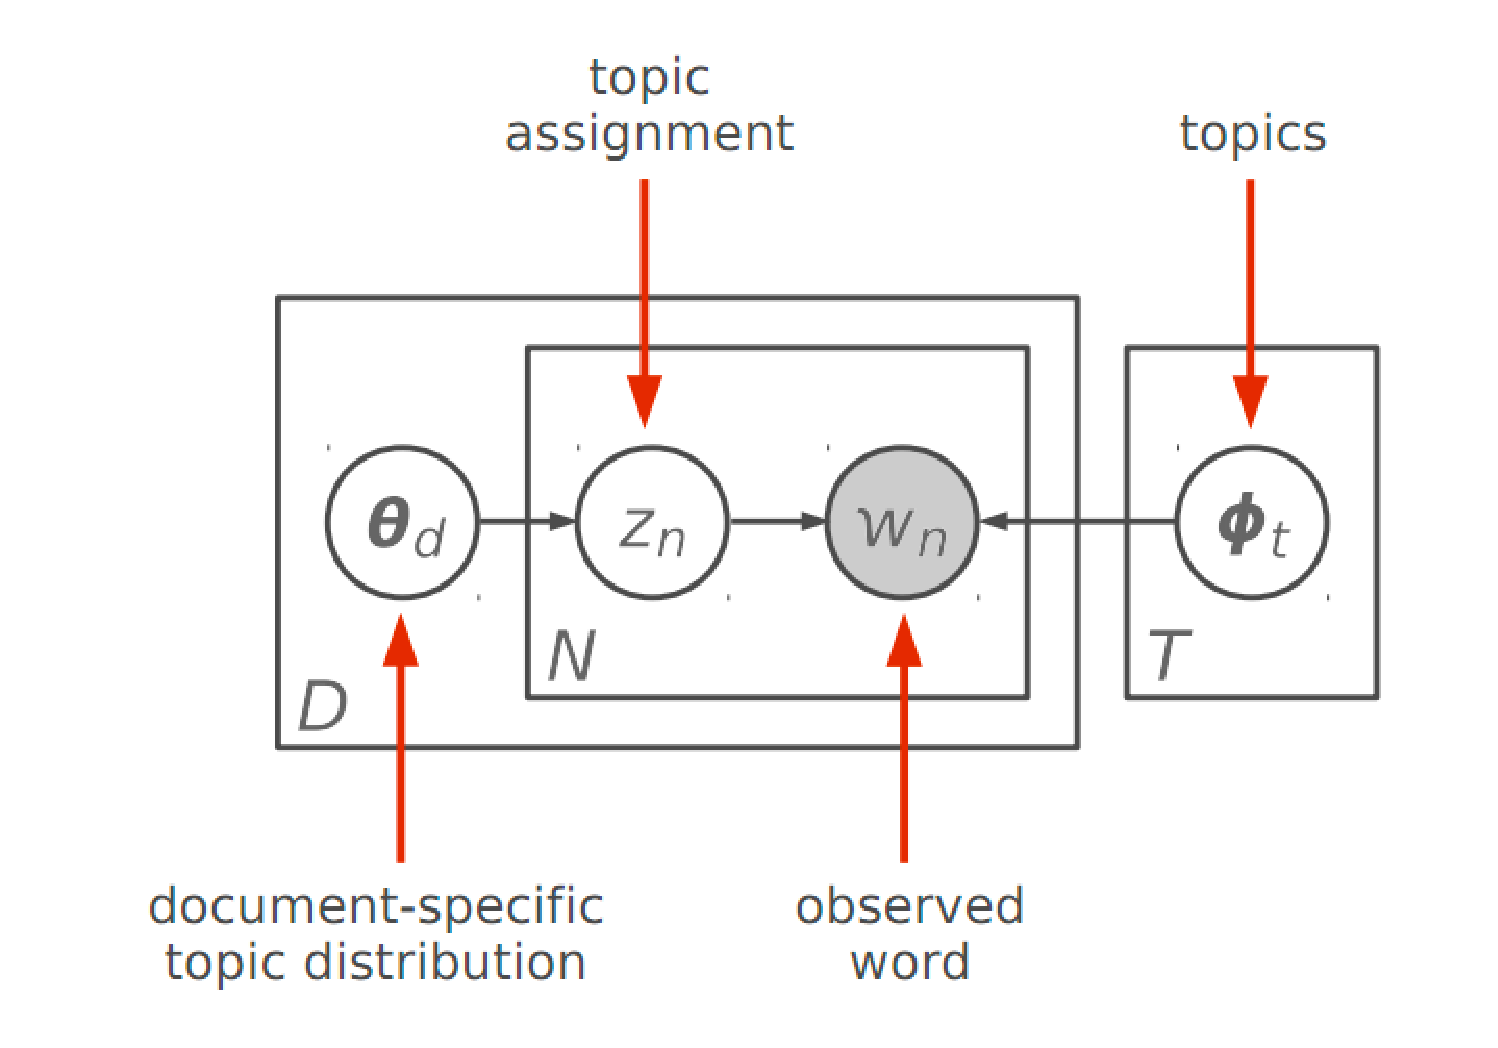
\includegraphics[width=400px]{figures/LSA.eps}
  \caption{The PLSA model}
  \label{fig:plsa}
\end{figure}

A significant step forward in this regard was made by Hofmann, who presented the probabilistic LSA (PLSA) model, where the mixture components are multinomial random variables that can be viewed as representation of “topics”~\cite{hofmann1999probabilistic}. Thus each word is generated from a single topic, and different words in a document may be generated from different topics. Each document is represented as a list of mixing proportions for these mixture components and thereby reduced to a probability distribution on a fixed set of topics. This distribution is the ``reduced description'' associated with the document. The PLSA model attempts to relax the simplifying assumption made in the mixture of unigrams model that each document is generated from only one topic. In a sense, it does capture the possibility that a document may contain multiple topics. 

\\
\item Latent Dirichlet allocation

Latent Dirichlet allocation (LDA) is a generative probabilistic model of a corpus and proposed by Blei David. The basic idea is that documents are represented as random mixture over latent topics, where each topic is characterized by a distribution over words. In LDA, it assumes the following generative process for each document to generate the words:

\begin{itemize}
\item Randomly choose a distribution over topics.

\item For each word in the document

  \begin {itemize}
\item Randomly choose a topic from the distribution over topics in step 1.
\item Randomly choose a word from the corresponding distribution over the vocabulary.
  \end{itemize}
\end{itemize}
\begin{figure}[!htb]
  \centering
  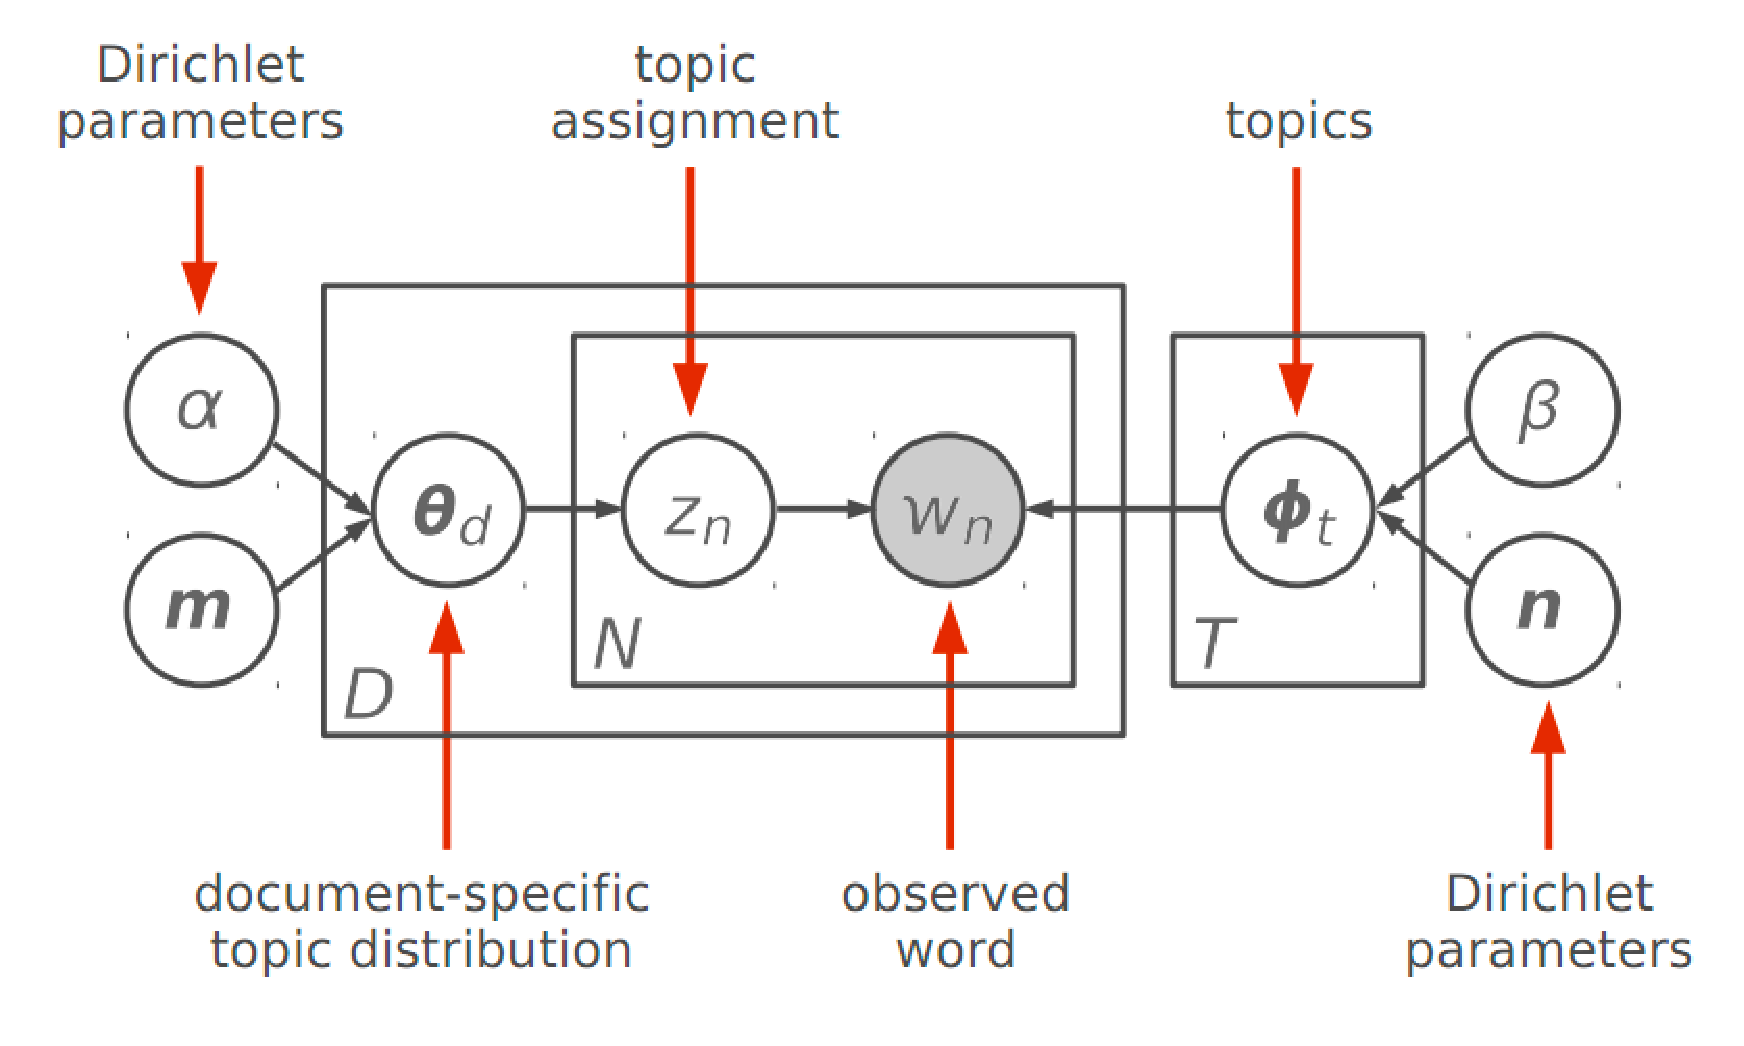
\includegraphics[width=400px]{figures/LDA.eps}
  \caption{The graphical model for latent Dirichlet allocation. Each node is a
random variable and is labeled according to its role in the generative
process. The hidden nodes–the topic
proportions, assignments and topics—are unshaded. The observed
nodes—the words of the documents—are shaded. The rectangles are
``plate" notation, which denotes replication. The N plate denotes the
collection words within documents; the D plate denotes the collection
of documents within the collection.}
  \label{fig:lds}
\end{figure}

This statistical model reflects the intuition that documents exhibit multiple topics. Each document exhibits the topics with different proportion; each word in each document is drawn from one of the topics, where the selected topic is chosen from the per-document distribution over topics. 
 
\end{itemize}

\section{Topology construction}
For some social medias, there are explicit social networks on which the information is diffused. This type of social medias includes the Twitter (the node represents the user, and the directed edge represents the following-followed relationship), Facebook (the node represents the user, and the undirected edge represents the friendship), etc. For the other social medias, we can only observe that one is got infected without knowing who infect it. This type of social medias includes the news websites and the personal blogs. We call this kind of topology construction prolem as network inference problem.

In~\cite{gomez2010inferring}, Gomez-Rodriguez et al. described this problem as: given a hidden directed network $G*(V,E*)$, where the set of $E*$ is unknown. Also for every node $v_i$, we know a triple tuple $(v_i,t_i,\Phi_i)$, which means at time $t_i$, $v_i$ is infected with a set of features or attributes $\Phi_i$. We aim to solve an optimization problem to find the set of $G*$. They built on the independent cascade model (See Chapter 4) and decribed the optimization problem as $$\hat{G} = argmax\limit_{|G|\le k}P(C|G)$$ where the maximization is over all graphs $G$ of at most $k$ edges.

In~\cite{eagle2009inferring}, Eagle et al. infered the friedship network structure from the mobile data and claimed that it is possible to accurately infer 95\% friendship relations.

In addition, some techniques to be introduced in Chapter 5.3 can be used to solve this problem.

\section{Sentiment analysis}
When analyzing the information diffusion, a very important attribute we need know is in which attitude a person got infected. Take the Twitter as an exmple, the users can rewteet a tweet with their comments. In this case, we can analyze the users' attitudes for the tweet by analyzing their comments. In~\cite{pang2008opinion}, Pang summaried 332 studies on opinion mining and sentiment analysis and classified the approaches into two categroies: the unsupervised approaches and supervised approaches. 

Among the unsupervised approaches, there ara a lot of studies on unsupervised lexicon induction, which is to create a sentiment lexicon in an unsupervised manner and use it to determine the degree of positivity of the content~\cite{hatzivassiloglou2000effects}~\cite{yu2003towards}. Bootstrapping is another unsupervised approach. The main idea is to generate the labeled data by using one available initial classifier~\cite{riloff2003learning}~\cite{wilson2005opinionfinder}. Moreover, Pang and Lee~\cite{thomas2006get} proposed a simple “blank slate” method based on the rarity of words within the search results that are retrieved. For the supervised approachs, they just use a collection of representative data to train a classifier. To compare these approaches, Chaovalit and Zhou did the comparing experiments on them~\cite{chaovalit2005movie}.









%\chapter{The diffusion models}
\label{chap:model}

The diffusion model is used for predicting the nodes that will be infected in the next time when given the structure and the infected nodes. First, we would like to introduce some basic states of the nodes. The classical disease-propagation model is based on a cycle of the individual’s status about the disease which we call SIR model. A person first is in susceptible (S) state which means he/she has the
chance to get infected when exposed to the disease by an infectious
contact. Then, the person will become infected (I). The disease runs
its course in that host, who is subsequently recovered (R).  A
recovered individual is immune to the disease for some period of time,
or for the rest of the whole life.  If the recovered individual
finally can become susceptible (S), we will call the model as SIRS model. 
Borrowed from the concept of the diease-propagation model, for the diffusion of the innovation, we can also treat the status of the individual as S, I, or R. Based on this concept, there are two diffusion models proposed: the threshold model and the cascade model. In this chapter, we will introduce these two widely used models that candecribe the process of the informaion diffusion.

\begin{itemize}

\item \textit{Threshold model}

In considering operational models for the spread of an idea or
innovation through a social network, represented by a directed
graph, we will say each individual node being either active (an
adopter of the innovation) or inactive. We will focus on the setting that
each node's tendency to become active increases monotonically as more
of its neighbors become active. Granovetter was
the first to propose models that capture such a process~\cite{granovetter1978threshold}. The
approach is based on the use of node-specific thresholds. 

Now we'd like to give a formal definition of the threshold  model: Given a directed graph $G=(V,E)$, for every $v_i \in V$, it chooses a threshold $\theta_{v_i}$ uniformly at random from the
 interval $[0,1]$ and it has two states: active or inactive. For every edge $(v_i,v_j) \in E$, it has a weight value denoting as $w(v_i,v_j)$. For every node $v_i$, we also calculate 
$b_{v_i}$ such that $b_{v_i} = \sum\limits_{(v_j,v_i)\in E \cap v_j\,is\,active}w(v_j,v_i)$.
 The process then proceeds as follows: given an initial set of
 active nodes $V_0$, the diffusion process unfolds deterministically in
 discrete steps: in step $t$, all nodes that were active in step $t-1$
 remain active, and we activate any node v for which the total weight
 of its active neighbors is at least $\theta_{v_i}$.
Thus, the thresholds $\theta_{v_i}$ intuitively represent the different
latent tendencies of nodes to adopt the innovation when their
neighbors do. However, as we are lack of the prior knowledge of their
value, we are in effect averaging over possible threshold values for
all the nodes.  

\item \textit{Cascade model}

Just like the threshold, we also consider the model based on a
directed graph. However, for the cascade model, whenever a node is
active, all of its neighbors have the probability that can be active.  

\end{itemize}

In ~\cite{kempe2003maximizing}, it is shown that the threshold model and the cascade model can be generalized and their generalized versions are the same. Actually, those two models just describe two different aspects of the social interaction. In the cascade model, it focuses on the individual interaction and the influence, while in the threshold model, it focuses on the threshold behavior: one will buy a new thing as long as there are enough friends buy it.  

Besides those two models, both of which are based on the direceted graph, there exist some models that are not based on the graph. In~\cite{yang2010modeling}, Yang et al. argued that in most cases, we cannot directly observe the structure of the network, which means the network over which the diffusion takes place is implicit or unknown. Thus, they proposed a Linear Influence Model (LIM) by constructing an influence function which has no relation with the individual node and only evaluates the total influence of the diffusion process at a given time.   

%\chapter{Research problems on social media}
\label{chap:direction}
In recent years, the research on social network in data mining area
is becoming more and more popular. Generally, the researchers are
interested in the following problems which are related to the
information diffusion: 1) influence maximization;
2) community Detection; 3) link prediction. In this chapter, we will
survey state-of-the-art work of the research on this three problems.

\section{Influence maximization}

The influence maximization problem is to find a group of nodes, which
we can call them influential nodes, as the seeds to maximize the
influence. 

Kempe et al.~\cite{kempe2003maximizing} studied the influence
maximization problem using two basic models, namely, the
independent cascade model and linear threshold mode. They proved that
this maximization problem under both the linear threshold model and
independent cascade model is NP-hard and proposed a greedy
alogrithm. The data they used is a collaboration graph which is
obtained from the co-authorship in physics publications. From the
experiment, they showed that the greedy algorithm significantly
outperformed the high-degree and centrality heuristics, which is
consistent with the conclusion drawn in the sociology literature. Also,
they mathematically proved that the greedy algorithm is a
$(1-e^{-1})$-approximation algorithm by using an analysis framework
based on submodular functions.

Based on the submodularity property of the maximization problem,
Leskovec et al. proposed a new greedy
algorithm called CELF, which is short for ``Cost-Effective Lazy Forward''~\cite{leskovec2007cost},
guaranteeing at least a constant fraction of the optimal
solution. In addition, they claimed that CELF could be as 700 times
fast as the simple greedy algorithm. They used this algorithm for the Battle of Water Sensor Network (BWSN), which is to
find the best sensor placements for a water distribution network in a real metropolitan area. Also, they did the experiment on blog data
to show the performance of the algorithm.

Chen et al. in their work~\cite{chen2009efficient} further improved
the greedy algorithm and called the new algorithm MixedGreedy and NewGreedy. The data they
used is the same as ~\cite{kempe2003maximizing}. The improvement
of the NewGreedy is to remove the edges that won't contribute to the
diffusion any more. MixedGreedy combines the CELF and NewGreedy
together: at the first round, the NewGreedy is applied and for the
rest, the CELF is applied. Another major contribution of their work is
that they presented a heuristic algorithm called DegreeDiscount which is
significantly faster than the greedy algorithm. However, it cannot
guarantee the constant factor of the optimal result.

Masahiro Kimura et al.~\cite{kimura2010extracting} proposed a method
of efficiently estimating all the marginal influence degrees of a
given set of nodes on the basis of bond percolation and graph theory,
and applied it to approximately solve the influence maximization
problem by the greedy algorithm. They used large-scale real
networks (i.e. blog networks) to demonstrate that the proposed
 method was much more efficient than ~\cite{kempe2003maximizing}.

\section{Community dectection}

The problem of community dectection is how to group the nodes in one social network together based on some particular properties of the nodes or some strategies.

Generally, there are two structures of the community: the overlapping community structure and the non-overlapping community structure. The overlapping community structure means for every node in the graph, i can belong to more than one communities and the non-overlapping community structure means for every node it can belong only one communities. 

Blondel et al. have analyzed a network of mobile phone communications between users of a Belgian phone operator~\cite{blondel2008fast}.
The vertices of the graph are 2.6 millions and the edges are weighted by the cumulative duration of phone calls between users in the observation time frame. The clustering analysis, performed with a fast hierarchical modularity optimization technique
developed by the authors, delivers six hierarchical levels. The highest level consists of 261 groups
with more than 100 vertices, which are clearly arranged in two main groups, linguistically homogeneous, reflecting the
linguistic split of Belgian population. 

Tyler et al.\cite{tyler2005mail} studied a network of e-mail exchanges between people
working at the HP Labs. They applied the same modified version of the Girvan-Newman algorithm that two of the authors have used
to find communities of related genes~\cite{wilkinson2004method}. The method enables one to measure the degree of membership
of each vertex in a community and allows for overlaps between communities. The detected clusters matched quite closely
the organization of the Labs in departments and project groups, as
confirmed by interviews conducted with researchers.

\begin{figure}[!htb]
  \centering
  \includegraphics[width = 340]{figures/community.eps}
  \caption{Community structure of a social network of mobile phone
    communication in Belgium. Dots indicate subcommunities at the
    lower hierarchical level (with more than 100 people) and are
    colored in a red–green scale to represent the level of
    representation of the two main languages spoken in Belgium (red
    for French and green for Dutch). Communities of the two larger
    groups are linguistically homogeneous, with more than 85\% of
    people speaking the same language. Only one community (zoomed),
    which lies at the border between the two main aggregations, has a
    more balanced distribution of languages.~\cite{blondel2008fast}}
  \label{fig:community}
\end{figure}


Traud et al.~\cite{traud2008community} used
anonymous Facebook data to create networks of friendships between students of different American universities, where
vertices/students are connected if they are friends on Facebook. Communities were detected by applying a variant of
Newman's spectral optimization of modularity: the results were further
refined through additional steps. One of the goals of the study was to
infer relationships between the online and offline lives
of the students. By using demographic information on the students' populations, one finds that communities are organized
by class year or by House (dormitory) affiliation, depending on the university. 

Yuta et al.~\cite{yuta2007gap} observed a gap in the
community size distribution of a friendship network extracted from mixi (mixi.jp), the largest SNS in Japan (as of December 2006). Communities were identified with the fast greedy modularity optimization by~\cite{clauset2004finding}.
Yuta et al. introduced a model where people form new friendships both by ``closing'' ties with people who are friends of friends, and by setting new links with individuals having similar interests. In this way most groups turn out to be either small or large, and medium size groups are rare.

\section{Link prediction}

For some social networks, while it is often possible to directly
observe when nodes become infected, observing individual transmissions
may be very difficult. The reason is that people cannot only get the
information from the social network, but also get it from offline
activity (e.g. a conversation) or other media. Also, we want to predict
which nodes will be infected in the future. We call those two problems
together as the link prediction problem. 

Liben-Nowell and Kleinberg proposed one of the earliest link
prediction models that works explicitly on a social network~\cite{liben2003link}. Every
vertex in the graph represents a person and an edge between two
vertices represents the interaction between people. They
concentrated mostly on the performance of various graph-based
similarity metrics for the link prediction task. Hasan et al. extended
this work in two ways~\cite{al2005link}: 1) using the external data
outside of the scope of the graph topology; 2) using various
similarity metrics as the features in a supervised learning setup. 

The link prediction problem has also been studied previously in the context
of relational data and also in the Internet domain, where explicit graph representations were not used. The prediction system proposed in
these works can accept any relational dataset, where the objects in the dataset
are related to each other in any complex manners and the task of the system is
to predict the existence and the type of links between a pair of objects in the
dataset. Probabilistic relational models, graphical model, stochastic relational models, and different variants of these are the main
modeling paradigm used in these works. The advantages of these approaches
include the genericity and ease with which they can incorporate the attributes
of the entities in the model. The disadvantage is that they are usually complex, and
have too many parameters, many of which may not be that intuitive to the user.

The research on social network evolution closely resembles the
link prediction problem. An evolution model predicts the future edges of a network, taking into account some well known attributes of social networks, such
as the power law degree distribution and the small world phenomenon.
This remains the main difference between evolution models and the link prediction models. The former concentrate on the global properties of the network
and the latter model the local states of the network to predict the probability of
the existence of a link between a special pair of nodes in the network. Nevertheless, the ideas from these models have been instrumental for some research
works that directly addressed the task of link prediction.

One of the main challenges of link prediction concerns the evolution of Internet scale social networks like Facebook, MySpace, Flickr, and so on. These
networks are huge in size and highly dynamic in nature for which earlier algorithms may not scale and adapt well. More direct approaches are required to
address these limitations. For instance, Tylenda et. al. shows that utilizing
the time stamps of past interactions, which explicitly utilize the lineage of interactions, can significantly improve the link prediction performance~\cite{tylenda2009towards}. Recently,
Song et. al. used matrix factorization to estimate similarity between the
nodes in a real life social network having approximately 2 millions nodes and
90 millions edges~\cite{song2009scalable}. Any traditional algorithm that aims to compute pair-wise
similarities between vertices of such a big graph is doomed to fail. Recently,
the matrix based factorization works have been extended to the more richer
higher-order models such as tensors.

%\chapter{The visualization techniques}
\label{chap:visualization}

In this chapter, we will survey current existing works on the
visualization of the information diffusion. Generally, most of
the work about the visualization is how to visualize the social
network. Also, there are some papers talking about spreading of the
disease which is similiar to information diffusion. At the last of the
chapter, we will summarize some visualization techniques that could be
used in information diffusion.

\section{Social network visualization}

There are already some surveys about visualizing the social
networks~\cite{freeman2000visualizing}
~\cite{correa2011visualizing}. 
In \cite{correa2011visualizing}, Correa gave a taxonomy of
visualization of the social networks. He classified the
visualization of the social networks into four main groups: structural
visualization, semantic visualization, temporal visualization, and
statistical visualization. Now we will explain these four groups in
detail:

\textit{Structural visualization}:

\begin{figure}[!htb]
  \centering
  \includegraphics[width = 300px]{figures/nodelink.eps}
  \caption{An example of node-link method for the structure
    visualization ~\cite{heer2005vizster}}
  \label{fig:nodelink}
\end{figure}

\begin{figure}[!htb]
  \centering
  \includegraphics[width = 500px]{figures/edgebundle.eps}
  \caption{Figure (a) shows the raw edges of the graph, and Figure (b) shows the result after the edge bundling.}
  \label{fig:edgebundle}
\end{figure}


The structural visualization focuses on how to visualize topology of a
graph extracted from a social network. Basically, there are two
different methods: the node-link method and the matrix method.

The node-link method is a very straightforward method that visualizes the
topology of the graph. As the real social network is ususaly very
huge, and it grows in complexity and size, a serious challenge for us
to visualizing it is how to find a good layout algorithm. Currently,
there are some techniques on graph visualization, which can be very
helpful for us to solve this problem. For example, in~\cite{holten2006hierarchical},
Holten proposed the hierarchical edge bundling algorithm to reduce the visual clutter (See Figure~\ref{fig:edgebundle}).

The matrix-oriented method is to represent a social network via an
explicit display of its adjacency or incidence matrix. In this
visualization, each link is represented as a grid location with
cartesian coordinates corresponding to the nodes in the
network. Color and opacity are often used to represent important
structural or semantic quantities. Consequently, a visual
representation of the adjacency matrix is much more compact than a
node-link method and overlap-free, since each link is represented
without overlap.

These two methods are indeed complementary. Thus, combining them
together is a good choice, which we call the hybrid method. The work done by Henry et al. is a very
typical example of the hybrid method~\cite{henry2007nodetrix}. They
proposed a new visualization called NodeTrix, using the node-link
method to visualize the overall structure of the network and using the
adjacency matrices to show the commnunities(See Figure~\ref{fig:nodetrix}).
Besides, the visualizations ~\cite{shen2007path} and
~\cite{muelder2008rapid} are also the hybrid methods.

\begin{figure}[!htb]
  \centering
  \includegraphics[width = 400px]{figures/nodetrix.eps}
  \caption{NodeTrix Representation of the largest component of the InfoVis Co-authorship Network ~\cite{henry2007nodetrix}}
  \label{fig:nodetrix}
\end{figure}

\textit{Semantic visualization}

Instead of highlighting the explicit relationships found in the data,
the semantic visualization focuses on representing the high level
attributes and connections of the nodes either as specified
explicitly in the data, or implicitly inferred from cross-referencing
externa sources.

Shen et al. proposed a visualization called OntoVis~\cite{shen2006visual} based on the
node-link method with a high-level graphical representation of the
ontology (See Figure \ref{fig:ontovis}).

\begin{figure}[!htb]
  \centering
  \includegraphics[width = 400px]{figures/ontovis.eps}
  \caption{Visualization of Terrorist Attacks (in green) Related to Hamas in 2005. Bombing is also the major tactic used by Hamas. However, their attacks focus on private citizens and properties. ~\cite{shen2006visual}}
  \label{fig:ontovis}
\end{figure}

\textit{Temporal visualization}:

The temporal information actually is a special type of high level
atrributes of the nodes or the edges in the graph. Since the social
interaction is a time-dependent phenomenon, it is only natural to
represent the temporal dimension visually. One of the
difficulties to represent time is a shortage of dimensions to depict a
dynamic network in a 2D display. As an alternative, one can represent
time along precisely one temporal demension. 

\textit{statistical visualization}:

The analysts are often interested in some statistical information,
which helps them to have an overview of the whole data and explore what
they need. This is at the core of visual analytics. The variables
often correspond to network statistics that represent the structure of
the network, such as degree, centrality~\cite{freeman1979centrality} and the clustering
coefficient. The first two describe the importance across the network,
the latter metric indicates how clusterable the nodes are in the social
network. 

\begin{figure}[!htb]
  \centering
  \includegraphics[width = 300px]{figures/plotmatrix.eps}
  \caption{An example of node-link method for the structure visualization ~\cite{dwyer2006visual}}
  \label{fig:plotmatrix}
\end{figure}

\begin{figure}[!htb]
  \centering
  \includegraphics[width = 350px]{figures/3dpc.eps}
  \caption{3D parallel coordinates for Padgett’s Florentine families marital relation data ~\cite{dwyer2006visual}}
  \label{fig:dpc}
\end{figure}


In general, network statistics form an N-dimensional space, where a
node or an edge is an observation, and each variable corresponds to an
attribute or metric. Dwyer et al. used a scatter plot matrix of common
centrality to understand the distribution of importance in social
networks~\cite{dwyer2006visual}, which is first used in
~\cite{koschutzki4comparison}. Dwyer et al. also used the 3D parallel
coordinates to represent the pairwise joint-distributions, which is to
represent each data point as a set of line segments whose endpoints
are the values of each of the variables (See Figure~\ref{fig:dpc}). Also, the scatter plots can
be used in representing the edge correlations. In
~\cite{goh2003betweenness}, Kahng et al. used this technique to study the
betweenness centrality correlation in social networks.

\section{Diffusion visualization}

\begin{figure}[!htb]
  \centering
  \includegraphics[width = 500]{figures/flu.eps}
  \caption{The Figure (a) shows the Pandemic Influenza Quick Look Tool
    Screenshot and Figure (b) shows the PanViz Applied at a National Level~\cite{brigantic2010development}}
  \label{fig:flu}
\end{figure}


To our best of knowledge, there is a lack of work on visualizing the
information diffusion for social networks. Nevertheless, Brigantic et
al. developed quick look tools (QLTs)  that can help the expert to clearly
see the Pandemic Influenza
modeling~\cite{brigantic2010development}. They claimed that, if an event 
happened, the QLTs could then be employed to rapidly assess and execute alternative mitigation strategies, and 
thereby minimize casualties.
 
\section{Other visualization techniques}

\begin{itemize}
\item Flow visualization

The information diffusion is just like the information flowing on the network. Thus, some techniques on flow visualization could be used. Flow visualization is a very big topic in scientific visualization
area and has being studied for many years. The flow visualization is about how to make flow pattern visible. In Figure. \ref{fig:flowvis} is an example.

\item Flow map
\begin{figure}[!htb]
  \centering
  \includegraphics[width = 300]{figures/flowvis.eps}
  \caption{Flow visualization of the ocean current in the Northeast Pacific using the Line Interval Convolution technique. Red indicates areas of high magnitude flowand blue indicates areas of low magnitude flow.~\cite{moorhead1995signal}}
  \label{fig:flowvis}
\end{figure}

The flow map is a visualization to visualize the network flow and the topology and shows the spatial distribution of univariate geographic phenomena. Generally, in a flow map, the width of the lines will represent the size of the flow, and we can merge edegs sharing the destinations in order to reduce the clutter. In ~\cite{phan2005flow}, Phan proposed a method that can generate the flow map automatically (See Figure ~\ref{fig:flowmap}c).

\begin{figure}[!htb]
  \centering
  \includegraphics[width = 500]{figures/flowmap.eps}
  \caption{Flow maps. (a) Minard’s 1864 flow map of wine exports from France. (b) Tobler’s computer generated flow map of migration from California from 1995 - 2000. (c) A flow map produced by our system that shows the same migration data.~\cite{phan2005flow}}
  \label{fig:flowmap}
\end{figure}

\item Trajectory visualization
\begin{figure}[!htb]
  \centering
  \includegraphics[width = 270]{figures/tra.eps}
  \caption{The visualization to show the aircrafts' traffic over France in one day. The color represents the altitude of the aircraft: the green represents the lowest altitude and the blue represents the highest altitude~\cite{hurter2009fromdady}.}
  \label{fig:tra}
\end{figure}

\begin{figure}[!htb]
  \centering
  \includegraphics[width = 300]{figures/tra2.eps}
  \caption{The visualization to show the density of the Dutch coast.\cite{willems2009visualization}}
  \label{fig:tra2}
\end{figure}

Trajectory visualization is trying to visualize the objects' movement based on their geographic information. There are several similarities between the diffusion visualization and trajectory visualization: 1) the data of the diffusion and the trajectory in temporal and spatial; 2) both the diffusion and the trajectory are based on the graphs. One of the major differences is that for the trajectory data, the geographic position is a key information to visualize. However, for the data of information diffusion on soical media, in most situation, there will be no geographic information. Thus, if we want to use the technology for the trajectory visualization, this is the importance issue that we should consider. Figure~\ref{fig:tra} and Figure~\ref{fig:tra2} are the examples for the trajectory visualization.

\end{itemize}

%\chapter{Conclusion and future work}
\label{chap:conclusion}

\section{Conclusion}
In this survey, we first reviewed the diffusion of innnovation theory. Then we introduced the three classical problems: influence maximization, community detection, and link prediction. According to the gerneral order of data mining procedures, we introduced the preprocessing techniques for the colleceted social media data, the models describing diffusing process, the proposed algorithms, and the mining results of those three problems. In the last, we introduced serveral studies on visualizing the social network and diffusion process. We also surveyed some highly related visualization techniques which could be used for future work. 

The diffusion of innovation on social media currently is still a very hot topic in different areas: The econimists are trying to study the strategies of advertising; The sociologists are trying to study the individual behaviours as well as social behaviours for the social network. Data mining techniques are very powerful for processing the large scale of data and finding what we want like the most influential nodes. However, the data mining techniques cannot meet all our needs: a) Are there some unsual patterns when the diffusion happens? b) How should we inspect the diffsuion process on the network? Moreover, a common problem of the data mining techniques is how we could help users including the experts in other fields to understand the mining results. 

\section{Future work}

As we illustrated before, the visualization techniques have shown great power for users to quickly understand massive data and inspect patterns. However, so far, there are few visualization tools which can show the diffusion process on the social network. Thus, designing a new visualization for the information diffusion on social media is critical. Besides, in order to let users easily understand the data as well as  the mining results, just a new visualization is not enough: a visual analysis system is needed.

For this new visualization, first, we should consider, which information should be encoded as the node position for the graph. As in many cases in social networks, we usually don't have or need geographic information, but people are very sensitive to the position of a node. In addition, for visualizing the information diffusion on the social network, in order to make it easy for users to understand the trend of the diffusion, the positions of the nodes are important. Second, we need to consider in which form we should encode the temporal information. Although there are some visualizations that try to visualize the temporal information, they may not be suitable for our cases and the effects are not good enough. Third, as the data acquired from the social media are in a huge scale, the scalability of the visualization should be seriously concerned. For example, we could design multiple visualizations to visualize the data in different levels of details. 


For the visual analysis system, we should focus on two things: 1) how to visualize the mining results; 2) how to design the user interactions. As making users better understand the mining result, such as the top influencers and the communities, we should further encode the information that why the data mining techniques return such the results, which would greatly help the users to know the rationality of the results. Besides, we should consider the overlapping problems when we want to visualize the multiple mining results. The user interactions are designed to make it possible for the user to manipulate the data including the raw data, the preprocessed data and the mining results. For the raw data, we should allow users filtering and reloading operations; For the preprocessed data, considering the accuracy problems of the text mining, we should allow users refining the data, such as the structure of the network, the topic of the text and the sentiment of text (negative or positive). For the mining results, we'd better provide two ways for users: 1) modifying the parameters of the mining models then running the mining algorithm again; 2) modifying the mining result directly. 










\bibliographystyle{theapa}
\bibliography{reference}
\end{document}
